\section{Мета роботи}
Освоєння аналітичних методів аналізу трудомісткості обчислювальних алгоритмів.


\section{Завдання}
\begin{enumerate}
    \item З табл. 1.2 обрати логічну схему алгоритму (ЛСА) відповідно до
    варіанта.

У ЛСА символам «Поч.» і «Кін.» відповідають початковий і кінцевий
оператори алгоритму. Символами A, B, C, D, E, K, M позначені
функціональні оператори алгоритму. Символами x1, x2, x3, x4 позначені
логічні умови. Якщо логічна умова дорівнює одиниці, то виконується
наступний один оператор у ЛСА. Якщо логічна умова дорівнює нулю, то
здійснюється перехід за стрілкою з відповідним індексом, у цьому випадку
у логічної умови стрілка спрямована уверх (наприклад, $\uparrow^i$). У місці переходу
з логічної умови стрілка спрямована вниз – $\downarrow^i$.
    \item За ЛСА побудувати графічну схему алгоритму, граф алгоритму та мінімальний граф алгоритму.
    \item Визначити трудомісткість алгоритму методами теорії марковських ланцюгів.
    \item Визначити середню трудомісткість алгоритму за допомогою
    мережевого підходу. Спочатку, якщо в алгоритмі є цикли, визначити
    середню трудомісткість циклів.
    \item Обчислити мінімальну і максимальну трудомісткість алгоритму.
    \item Проаналізувати отримані результати.
\end{enumerate}

\begin{figure}[ht!]
    \centering
    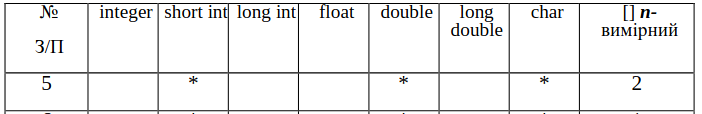
\includegraphics[width=.7\textwidth]{\assetsDirectory/var.png}
    \caption{Завдання за варіантом (\variant)}
\end{figure}

\begin{figure}[ht!]
    \centering
    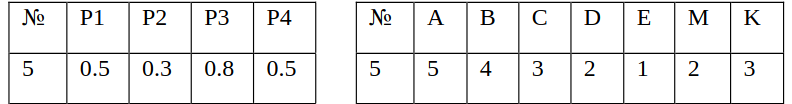
\includegraphics[width=.7\textwidth]{\assetsDirectory/var1.png}
    \caption{Завдання за варіантом (\variant)}
\end{figure}

\newpage
\section{Хід роботи}
\subsection{За ЛСА будуємо графічну схему алгоритму, граф алгоритму та мінімальний граф алгоритму}
\begin{figure}[ht!]
    \centering
    \subfigure[]{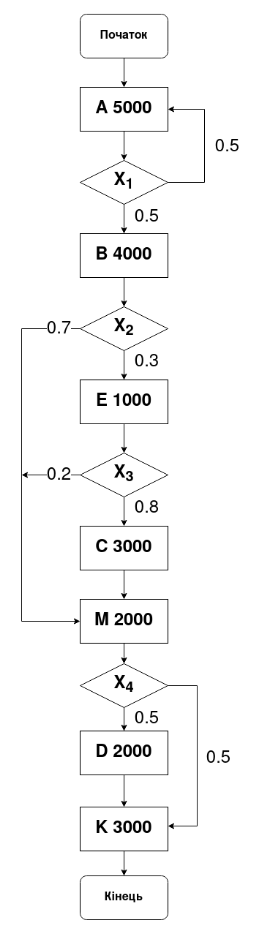
\includegraphics[height=18cm]{\assetsDirectory/diag1.png}} 
    \subfigure[]{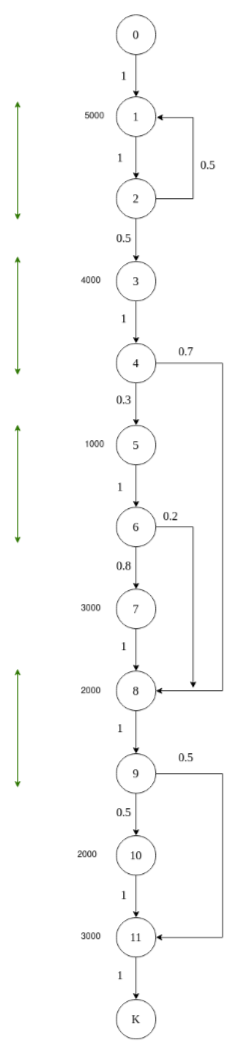
\includegraphics[height=18cm]{\assetsDirectory/diag2.png}} 
    \subfigure[]{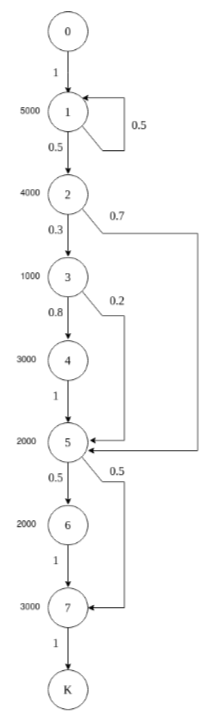
\includegraphics[height=18cm]{\assetsDirectory/diag3.png}}
    \caption{(а) графічна схема алгоритму (б) граф алгоритму (в) мінімальний граф алгоритму}
\end{figure}


\newpage
\subsection{Визначаємо трудомісткість алгоритму методами теорії марковських ланцюгів}

\begin{figure}[ht!]
    \centering
    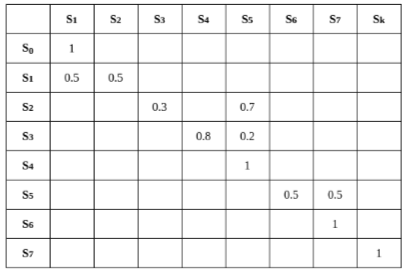
\includegraphics[width=.7\textwidth]{\assetsDirectory/mark.png}
    \caption{Стахостична матриця}
\end{figure}

\noindent
Обчислення кількості звертань до вершин:\\
$n_0 = 1$\\
$n_1 = 1 * n_0 + 0.5 * n_1 | n_1 - 0.5 * n_1 = 1 | n_1 = 2$\\
$n_2 = 0.5 * n_1 = 1$\\
$n_3 = 0.3 * n_2 = 0.3$\\
$n_4 = 0.8 * n_3 = 0.24$\\
$n_5 = 0.7 * n_2 + 0.2 * n_3 + n_4 = 0.7 + 0.2 * 0.3 + 0.24 = 1$\\
$n_6 = 0.5 * n_5 = 0.5$\\
$n_7 = 0.5 * n_5 + n_6 = 0.5 *1 + 0.5 = 1$\\
$n_k = 1$\\

\noindent
Трудомісткість:\\
$\Theta = 10000 + 4000 + 300 + 720 + 2000 + 1000 + 3000 = 21020 \text{(оп)}$\\



\newpage
\subsection{Визначаємо середню трудомісткість алгоритму за допомогою мережевого підходу}

\begin{figure}[ht!]
    \centering
    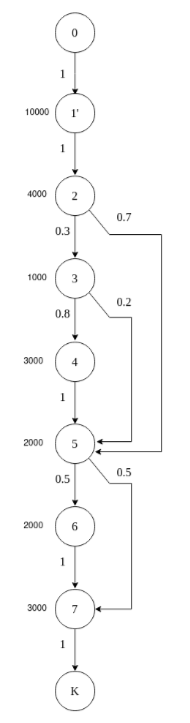
\includegraphics[width=.3\textwidth]{\assetsDirectory/net.png}
    \caption{Граф алгоритму без циклів}
\end{figure}

\newpage
\begin{figure}[ht!]
    \centering
    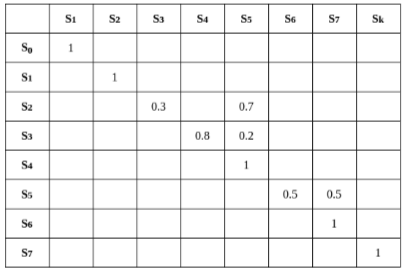
\includegraphics[width=.7\textwidth]{\assetsDirectory/net1.png}
    \caption{Стахостична матриця}
\end{figure}

\noindent
Обчислення кількості звертань до вершин:\\
$n_c = \frac{1}{1 - 0.5} = 2$\\
$q_c = n_c * q_{mc} = 2 * 5000 = 10000$\\

\noindent
Обчислення кількості звертань до вершин:\\
$n_0 = 1$\\
$n_1 = 1$\\
$n_2 = 1$\\
$n_3 = 0.3 * n_2 = 0.3$\\
$n_4 = 0.8 * n_3 = 0.24$\\
$n_5 = 0.7 * n_2 + 0.2 * n_3 + n_4 = 0.7 + 0.2 * 0.3 + 0.24 = 1$\\
$n_6 = 0.5 * n_5 = 0.5$\\
$n_7 = 0.5 * n_5 + n_6 = 0.5 *1 + 0.5 = 1$\\
$n_k = 1$\\

\noindent
трудомісткість:\\
$\Theta = 10000 + 4000 + 300 + 720 + 2000 + 1000 + 3000 = 21020 \text{(оп)}$\\


\newpage
\subsection{Обчислити мінімальну і максимальну трудомісткість алгоритму}

Для знаходження мінімальної та максимальної трудомісткісті алгоритму зобразимо на графі
максимальний та мінімальний шлях для проходження алгоритму, а позначимо їх зеленим кольором.
Але через те, що там є цикли,
то візьмемо для обрахунку максимальної трудомісткісті алгоритму візьмемо середні трудомісткісті циклів.

\begin{figure}[ht!]
    \centering
    \subfigure[]{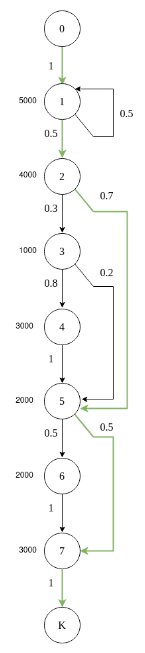
\includegraphics[height=16cm]{\assetsDirectory/min.png}} 
    \subfigure[]{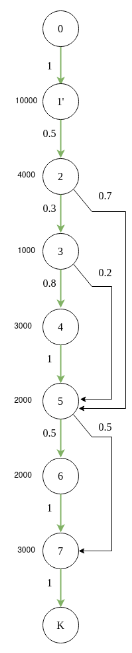
\includegraphics[height=16cm]{\assetsDirectory/max.png}} 
    \caption{(а) Мінімальний (б) Максимльний}
\end{figure}

\noindent
Максимальна кількість операцій: $25000 \text{(оп)}$\\
\noindent
Мінімальна кількість операцій: $14000 \text{(оп)}$

\newpage
\subsection{Висновки}
В ході виконання лабораторної робити було розглянуто 2 метода для обрахунку трудомісткість:
метод Марковський ланцюгів та мережевий метод. За допомогою них було вирахувано середню трудомісткість алгоритму,
та в результаті їх значення збігаються. Також було розраховано мінімальну та максимальну трудомісткість алгоритму.
